Data centers and HPC systems differ significantly in terms of their traffic characteristics. While the majority of traffic in a data center is small-scale, unpredictable, and not localized to any one level of the switch, traffic in an HPC application is primarily near-neighbor traffic, and may not be modest flows. Traditional flow identification methods may not be effective
in HPC environments. To effectively support SDN in the HPC environment,
novel techniques that take HPC communication characteristics into
consideration are proposed. Since a significant portion of
communications in HPC applications are static, we propose to have an API for
applications to provide flow information to the network directly. For
dynamic communications, we develop a machine learning based approach for
flow identification.

Figure~\ref{fig:flow_schemes} shows the high-level view of the proposed
flow classification systems. The flow classification techniques can
be classified into two types, those {\em with no extra user information} and
those {\em with user information}. The components below SDN API are similar to
traditional SDN systems. The flow classifier may take traffic statistics from
SDN switches and performs flow classification with no extra user information.
The classifier also allows HPC applications (SDN user) to directly give
hints about their communications to the network through an API
(similar to the intent-based API \cite{Coflow2012}), and classifies
such flows based on user information.

\begin{figure}[h]
\centering
    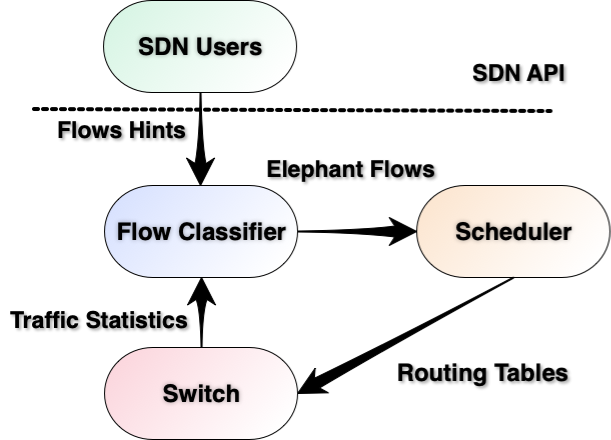
\includegraphics[width=0.8\columnwidth]{figs/Fig3.png}
\caption{High-level view of our flow classification schemes}
  \label{fig:flow_schemes}
\end{figure}

\subsection{Flow identification without user input}


\vspace{0.08in}
\noindent{\bf Threshold-based scheme}:
Existing flow classification methods including end host-based
management~\cite{xu2015identifying},
packet sampling~\cite{suh2014opensample}~\cite{afek2015sampling},
and polling per-flow statistics~\cite{yang2020flow}, do not assume
the type of applications. In this work, we compare our proposed techniques with
the classic elephant flow detection using a polling-based approach,
which is based on Hedera's architecture \cite{al2010hedera}.
Hedera's control loop comprises
three main components: flow detection, channel calculation, and channel
placement. Initially, significant 
flows are detected at the edge switches, and appropriate channels for these 
large flows are calculated using placement algorithms, taking into account 
their natural demand. These pathways are then placed on the switches.
%Hedera's architecture supports all common multi-rooted tree topologies.

Due to the overhead concerns, there is a limit how fast the flow statistics
are gathered, and path calculation and installations are performed, which is typically
in the order of seconds \cite{al2010hedera}.
However, in the HPC environment, depending
on applications, the time for each iteration may be much less than a second.
Hence, these existing flow classification schemes will miss many iterations
of application execution and not effective for such HPC applications.
To perform flow classification effectively for HPC systems, we develop
a machine learning based approach using deep neural network (DNN)
for flow classification.

\vspace{0.08in}
\noindent{\bf Deep learning-based scheme}:
As mentioned earlier, communications in HPC applications exhibits phase
behavior. If such behavior can be characterized and learned, we can classify
the flows quicker (after a small number of phases).
The information to differentiate between large elephant flows from
small mice flows is fundamentally captured by the time sequence of packets.
By training a Deep Neural Network (DNN) model using the time sequence of
packets from HPC workloads, the DNN model is able to recognize the
patterns of elephant flows in HPC applications. We note that the patterns
learned by the DNN model goes beyond simple statistics like
the existing threshold-based scheme: the model can also reflect more
sophisticated patterns such as the phased behavior. 


\vspace{0.08in}
\noindent{\em Model architecture}:
Our DNN model consists of an input layer of size 300 to accept the input data
which consists of data sent across various intervals of time and a single dense layer with
one output neuron, which uses the sigmoid activation function to classify the flows as elephants or mice.
The sigmoid function is commonly used for binary classification tasks
as it outputs a value between 0 and 1, which can be 
interpreted as the probability of the input belonging to the positive class. 
The model uses the Nadam optimizer with a learning rate of 0.01. Nadam is an 
extension of the popular Adam optimizer that incorporates Nesterov momentum, 
which helps to accelerate convergence. The model is compiled with binary 
cross-entropy loss, which is a standard loss function used for binary 
classification tasks.

\vspace{0.08in}
\noindent{\em Data collection and model training}:
We utilized the TraceR-CODES simulator to execute representative HPC 
workloads, namely Random-Permutation, Shift-256, Stencil3d, Stencil4d, Milc, Nekbone, Subcom3d-a2a, Kripke ~\cite{kripke}, Laghos, 
SW4lite ~\cite{sjogreen2018sw4}, and AMG ~\cite{amg}, 
for ranks ranging from 32 to 512. More detailed description of these
workloads is given in Section~\ref{sec:exp}.
Flow statistics were collected every 0.3 
seconds or 1\%
of the simulation to maintain minimal granularity. The flow data 
was gathered independently for each rank and merged to train the DNN 
model. For training purposes, the flows are marked as elephant or
mouse flows with a cut-off of $3 * 10^8$ bytes of data transfer in 90 seconds: 
Elephant flows were those transferring more than 300 MB of data in
90 seconds, while mouse flows were 
those transferring less. We employed a min-max scalar to scale the flow data 
before inputting it into the dense neural network layer for forecasting. The 
developed model was used offline to forecast network flows of elephants
or mice for systems running a combination of the aforementioned
applications.

During training, the model is trained on the input data and
corresponding binary labels. The total data is split as follows 20\%
of the training data is used for validation, while the remaining 80\% is 
used for training. Table~\ref{tab:model_acc} shows the model prediction
accuracy: the model prediction accuracy is very high for the data. 
We first trained the model on the applications which we are going to use for our simulations and 
see how it performed which are Random-Permutation, Shift-256, Stencil3d, Stencil4d, Milc, Nekbone and later on we added Subcom3d-a2a, Kripke , Laghos, SW4lite, and AMG for training to see if the model is able to handle the new data, along with the existing data and still provide a accurate prediction. We do this to make sure that our model is capable of getting  updated with new traffic as an when it comes. 

\begin{comment}
\paragraph{Model Offline Prediction}				
We conducted a study on three workloads generated by randomly selecting 
applications from Stencil4d, Subcom3d-a2a, Kripke, Laghos, AMG,
and SW4lite for  
ranks 32, 64, 128, 256, and 512. The TraceR-CODES simulator was used to 
simulate the corresponding workloads, and the flow data was collected.
The network flows that we gathered 
for the workload were predicted using the model. 

To validate the model's ability to forecast elephants and mice for any 
applications, we tested the model on unknown data. The model was employed to 
forecast the network flows of the application while it was operated 
individually and as a workload, and in each case, the model accurately 
predicted the flows by more than 95\%. The data used for making the 
predictions are presented in the table below.

Overall, our study demonstrates the effectiveness of the proposed neural 
network model for accurately predicting network flows of elephant and mice for 
various applications, which can assist in improving the performance of HPC 
systems.
%
\end{comment}

\begin{table}[h]
  \centering
  \caption{Accuracy of predicting elephants and mice flows by the DNN model for averaged across 32, 64, 128, 256 and 512 ranks}
    \label{tab:model_acc}
    \begin{tabular}{lr} \toprule
\multirow{1}{*}{Applications} & Accuracy \\ \midrule
Random-permutation & 100.0\\
Shift-256 & 100.0\\
Stencil3d & 100.0\\
Stencil4d & 100.0\\
Milc & 100.0\\
Nekbone & 100.0\\
\midrule
AMG & 100.0\\
Kripke & 100.0\\
Laghos & 100.0\\
Subcom3d & 100.0\\
SW4lite & 98.2\\ \bottomrule
\end{tabular}
\end{table}


\subsection{Flow identification with user input}

For static communications in HPC applications like the ones in Stencil4d
shown in Figure~\ref{code.stencil}, the HPC application developer (or
compiler and communication library) has
the knowledge whether a communication is an
elephant flow or not and can mark each flow in an MPI point-to-point
communication as elephant flow or a mice flow or all flows in an
MPI collective communication as elephant flows.
With this approach, the SDN basically passes the flow identification
task to the applications (done by application developer, compiler, or
runtime library), which greatly simplifies the SDN operation.

\begin{comment}
\textcolor{red}{
  The code indicates that each node sends eight communication messages to its neighbors. Additionally, since the neighbors are determined only during the compile time and the set of neighbors do not change during the runtime, user have the ability to correctly predict the communication characteristic. If the user knows the mapping of the ranks to nodes in the HPC system during the running of the application and also the data sent in the MPI calls, they can determine the communication characteristic of the application in the actual system and can determine which flows are elephants and which are mice when a HPC application starts running on a system.}
\end{comment}

There are different static communications in HPC applications. Consider
MPI applications. The most complete information about a point-to-point
communication includes the source MPI rank, the destination rank, and the
message size. The communications in Stencil4d belong to this type. 
For such communications, users can give the hint when the
application is loaded (when MPI ranks are mapped to physical nodes).
For communications whose source and destination cannot be determined
statically, but the size can be decided, the hints may be given at runtime
when the communications are executed.
The example of Laghos shown in Figure~\ref{code.laghos} belongs to this type. 
Such information can also be used
for collective communications where a group of processes are involved in
the communication.
In the case when message size cannot be determined, the user may still use the
API to indicate that a flow is an likely
elephant flow with the knowledge of the applications. The SDN may use a
simpler flow classification than the ones dealing with the most general
unknown flows.
 
\begin{comment}
Here, the system detects the elephant flows and checks
if it is marked by the user, if both marks the flows as elephant then the flow is regarded as elephant, however if the user indicated the flow wrongly, and the system, detects the flows as elephant flows for three or more consecutive intervals then the priority is given to the system clarification. Using user information, the system and the user work together
to identify flows and the flow identification at the network system level is
greatly simplified. 
  \textcolor{red}{ Figure~\ref{fig:complete_info} shows the Speedup with respect to D-mod-k routing for static applications for 256, 512 and 1024 ranks when users have the complete knowledge of the application characteristic. For Random permutation, having such knowledge beforehand offers a speedup of around 2 for 256 ranks. For larger ranks it still achieves a speedup around 1.5. For Stencil4d the approach provides a speedup of more than 1.4}


\begin{figure}[h]
  \centering
  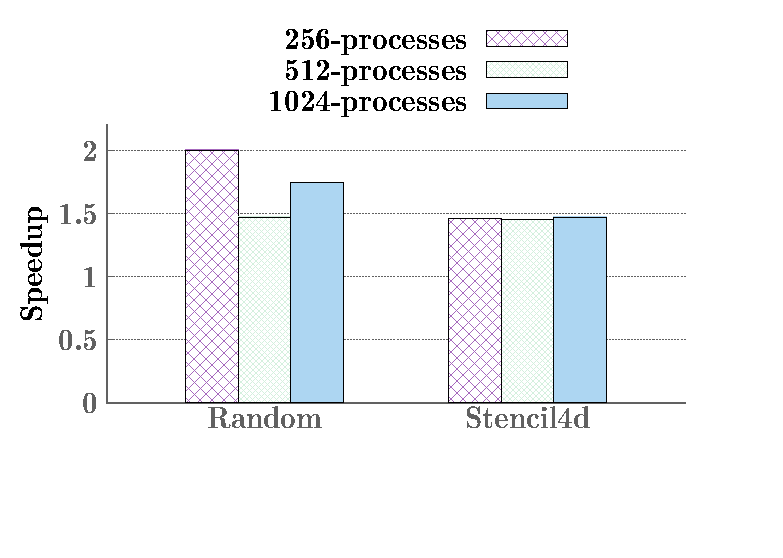
\includegraphics[width=\columnwidth]{./figs/scripts/plot_scripts/complete-info.eps}
  \caption{Speedup in latency for various techniques compared with D-mod-k for 
applications with static communication with user marked elephant flow only on fat-tree for 256, 512 and 1024 processes.}
  \label{fig:complete_info}
\end{figure}

\end{comment}

